% !TEX encoding = UTF-8 Unicode
\documentclass{article}

\usepackage{polski}
\usepackage[utf8]{inputenc}
\usepackage{subfig}
\usepackage{tikz}


\usepackage[a4paper, left=2.5cm, right=2.5cm, top=3.5cm, bottom=3.5cm, headsep=1.2cm]{geometry}

\linespread{1.3}
 
\begin{document}

\begin{titlepage}
\centering
{\scshape\LARGE Politechnika Wrocławska \par}
{\scshape\Large Katedra Informatyki Technicznej\par}

	\vspace{1cm}
	{\scshape\Large Inżynieria Oprogramowania\par}
	\vspace{1.5cm}
	{\huge\bfseries Wykonanie opisu biznesowego "świata rzeczywistego"\par}
	\vspace{2cm}
	{\Large\itshape Magdalena Biernat\par}
	{\Large\itshape Mateusz Bortkiewicz\par}
	\vfill
	Opiekun\par
	prof. dr hab. inż. Jan Magott 

	\vfill
	{\large \today\par}
\end{titlepage}
\newpage

\section{Wprowadzenie}
Sprawozdanie dotyczy drugich zajęć. Na tych laboratoriach zaczęliśmy swój projekt. 

\subsection{Cel laboratorium}
Stworzyć opis najważniejszych procesów biznesowych występujących w tzw. świecie rzeczywistym, które należy zautomatyzować za pomocą projektowanej aplikacji oraz specyfikację wymagań funkcjonalnych i niefunkcjonalnych tej aplikacji.

\subsection{Plan pracy}
Zadania wykonaliśmy wg instrukcji 2:
\begin{itemize}
\item Wybór tematu aplikacji.
\item Wykonanie opisu "świata rzeczywistego".
\item Zdefiniowane wymagań funkcjonalnych i niefunkcjonalnych. 
\end{itemize}
\section{Laboratorium}

\subsection{Wybór tematu aplikacji}
Wybraliśmy temat wypożyczalni płyt i kaset. Jako dodatkową opcję planujemy, żeby nasza aplikacja obsługiwała czytnik kodów kreskowych.

\subsection{Opis "świata rzeczywistego"}
Pracownicy wypożyczają płyty DVD, Blu-ray oraz kasety. Każda pozycja na magazynie posiada indywidualną liczbę porządkową, a także kod kreskowy. Posiada referencję do danego tytułu, nośnik, obecnego klienta, datę wypożyczenia oraz przewidywaną datę zwrotu. Pracownicy mogą również wprowadzić nowe artykuły do systemu, a także oznaczać jako uszkodzone (dokonywać ich usunięcia). System powinien automatycznie tworzyć dokumenty (faktury oraz dokumenty magazynowe) na podstawie wprowadzanych wypożyczeń i zwrotów. Pracownik może przeglądać stany magazynowe. Identyfikacji danej pozycji może dokonać za pomocą czytnika kodów kreskowych.

\subsection{Przepisy i strategia firmy}
Użycie systemu wypożyczeń w celu maksymalizacji zysków.

\subsection{Dane techniczne}
Użytkownicy systemu: 3-4 pracowników (praca wg ustalonego grafiku).
Pracownicy to studenci, którzy mogą poświęcić kilka/kilkanaście godzin w tygodniu. 
Tysiące artykułów do wypożyczenia, setki tytułów, różne nośniki (VHS, DVD, Blu-ray)
150 do 300 razy dziennie użyte dane do wypożyczenia (w zależności od dnia).

\subsection{Wymagania funkcjonalne i niefunkcjonalne}
\begin{itemize}
\item Program powinien wypożyczać kasety/płyty. Podawać termin oddania, Wyliczenie kosztu wypożyczenia. 
\item Wyliczanie kosztów w przypadku przetrzymania, wystawianie paragonu czy też faktury. Wystawianie dokumentów przyjęcia zewnętrznego i rozchodu wewnętrznego.
\item Wypożyczalnia wypożycza płyty/dvd osobom za okazaniem dowodu osobistego. Posiada podstawowe informacje nt. klienta, tj. imię, nazwisko, adres zamieszkania, telefon kontaktowy, adres skrzynki mailowej.
\item Wypożyczalnia dokonuje zakupu nowych płyt/kaset. Usuwa zniszczone płyty/kasety. 
\item Wypożyczający komunikuje się z klientem. 
\item Wypożyczającemu pomaga system.
\item Wypożyczalnia może edytować dane płyt/kaset i wypożyczających.
\end{itemize}

\subsection{Diagram wymagań}
Na podstawie wymagań z poprzedniego podpunktu, stworzono diagram wymagań w środowisku Visual Paradigm. Przedstawia się on następująco:
\begin{figure}[!ht]
\centering
	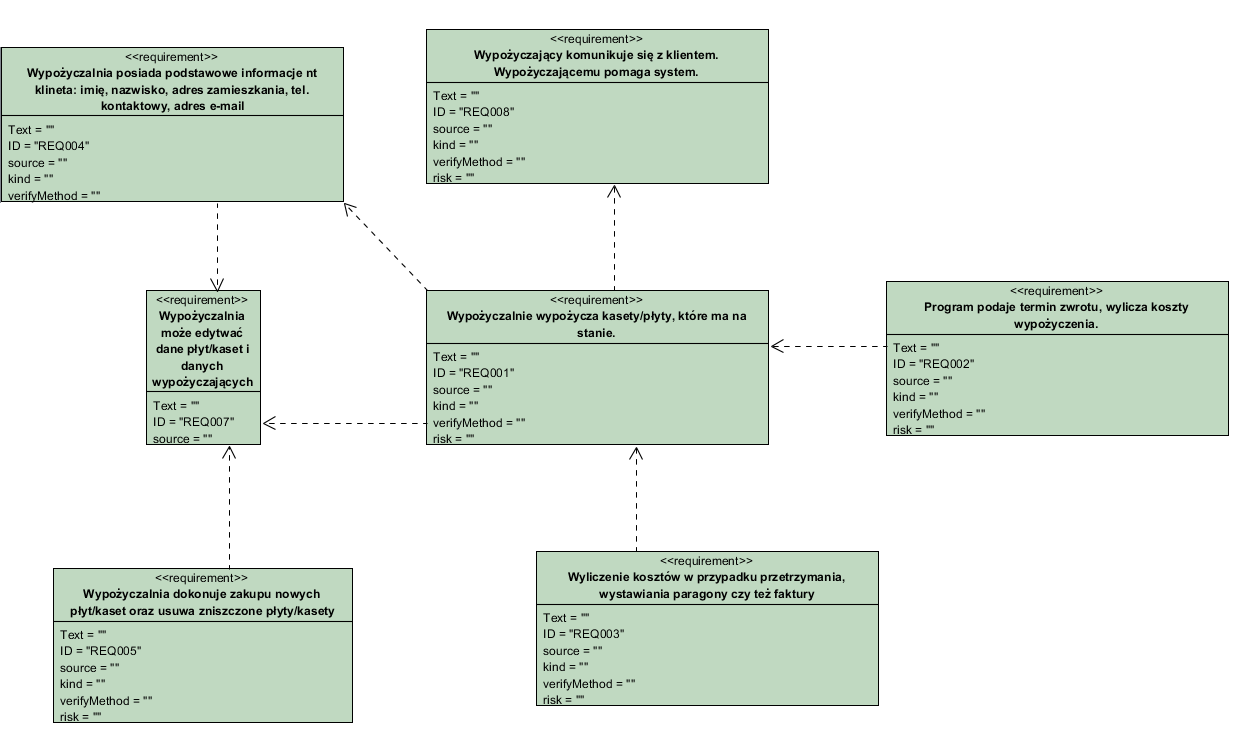
\includegraphics[width=16cm]{diagramwymagan.png}
	\caption{Diagram wymagań}
	\label{fig:obrazek 1}
	\end{figure}

\end{document}
